\section{Imagination Augmented Agent (I2A)} 
\label{sec:i2a} 
 
The paper "Imagination-augmented agents for deep reinforcement learning" from Weber et al. \cite{I2A} combines the advantages of model free and model based reinforcement learning to get an agent which is robost against model imperfections but is able to use the advantages of model based agents.
The imagination-augmented agent learns therefore to combine information from a model-free and a model-based imagination-augmented path.\\

%To do this they train a model of the environment for internal simulations. 
%Imagine the future and learn to do better actions based on the imagined future.\\ 
 
Figure \ref{fig:i2a_architecture} shows the network architecture of the imagination-augmented agent, which will be explained in the following.

\begin{figure}[H] 
  \centering 
   
  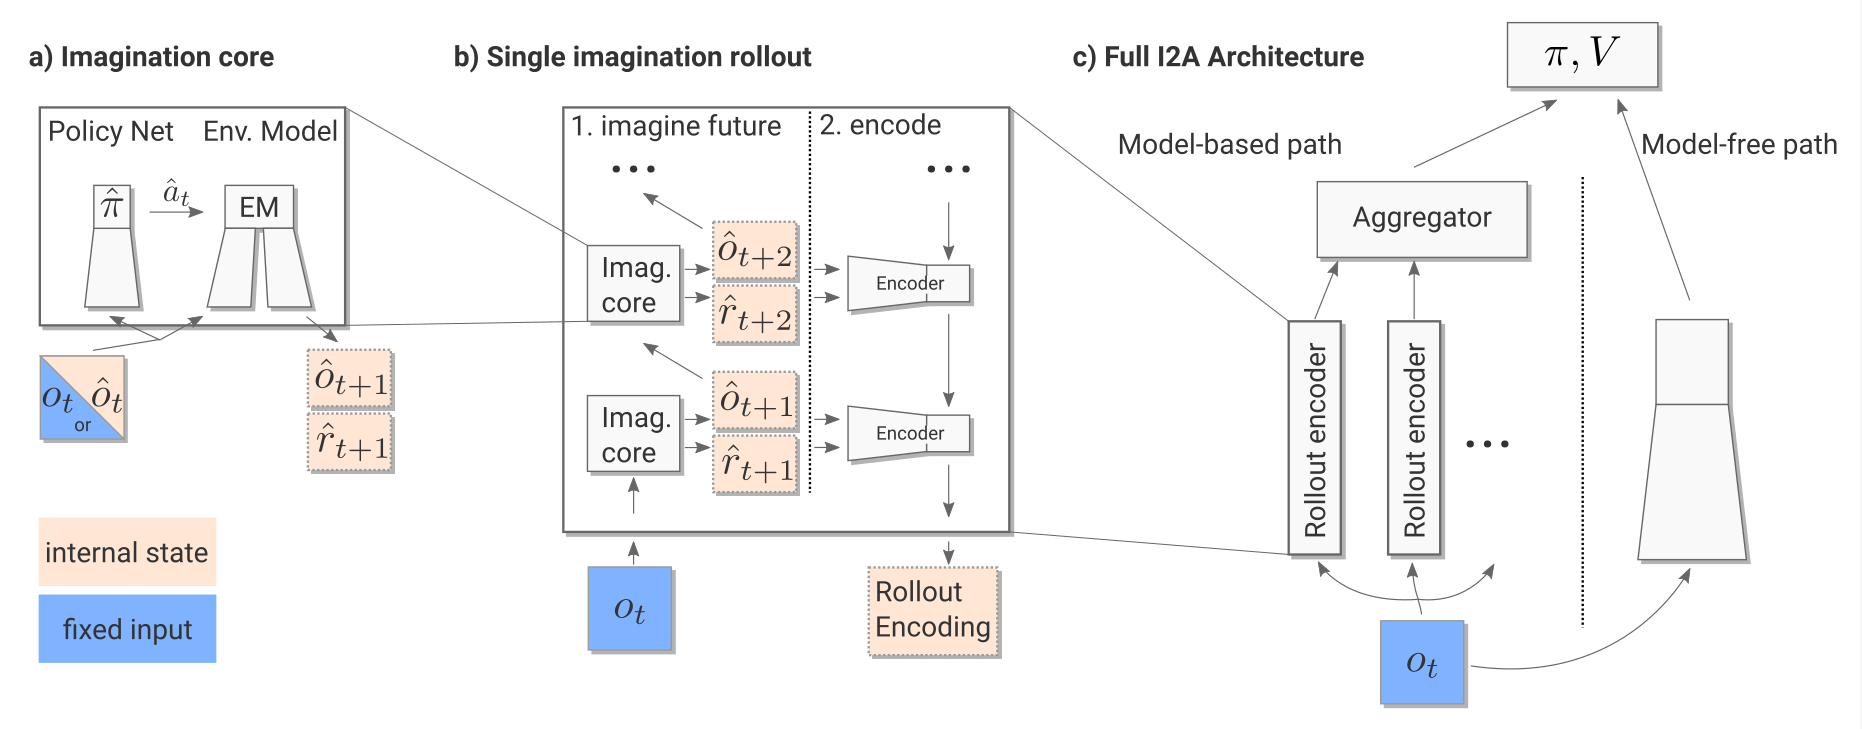
\includegraphics[width=\columnwidth]{./Images/i2a_architecture.png} 
  \caption{Network architecture for deep reinforcement learning which combines model free and model based reinforcement learning. a) imagination core (IC) predicts the next time step conditioned on an action sampled from the rollout policy $\hat{\pi}$. b) the from the imagination core imagines trajectories of features f encoded by the rollout encoder. c) the full i2a} 
  \label{fig:i2a_architecture} 
\end{figure} 
 
\subsection{Imagination core}

The \textbf{imagination core} (Figure \ref{fig:i2a_architecture} a)) imagine the next observation $\hat{o}_{t+1}$ and the next reward $\hat{r}_{t+1}$ given the observation $o_t$ or $\hat{o}_{t}$, where $o_t$ refers to the  input the i2a get and $\hat{o}_{t}$ refers to an internal state of i2a which is an output of a previouse rollout with the imagination core.
To do so the imagination core uses a rollout policy, which predict an action given the current state, and an environment model \ref{sec:env_model}, which predict the next observation and the next reward.\\

%$o_t$: initial observation  $\hat{o}_t$: predicted observation  $\hat{r}_t$: predicted reward Given observation $o_t$ or $\hat{o}_t$ and action $\hat{a}_t$ predict (imagine) the next observation $\hat{o}_{t+1}$ and next reward $\hat{r}_{t+1}$  

%To do so the imagination core uses a rollout policy, which decides the next action $\hat{a}_t$, and an environment model, which predicts the next state and the reward signals from the environment, given an state and a current action.\\


The \textbf{rollout policy $\hat{\pi}$} is a model-free reinforcement learning agent which should, given the same observation, predict the same action as the i2a policy. To ensure this, the rollout policy need to be similar to the i2a policy $\pi$, which can be ensure by minimizing the distillation loss, the cross entropy between the rollout policy $\hat{\pi}$ and the i2a policy $\pi$:

%Distillation loss Make $\hat{\pi}$ (rollout policy) and $\pi$ (i2a policy) similar\\ 
 
\begin{equation} 
    l_{dist}(\pi, \hat{\pi})(o_t) = \lambda_{dist} \sum_a \pi(a | o_t) log \hat{\pi}(a|o_t) 
\end{equation} 

with scaling parameter $\lambda_{dist}$.\\
% $\lambda_{dist}$ is set to 10



\subsection{Environment Model (EM)}
\label{sec:env_model}

The environment model predict (imagine) the next observation $\hat{o}_{t+1}$ and next reward $\hat{r}_{t+1}$, given observation $o_t$ or $\hat{o}_t$ and action $\hat{a}_t$.\\

It is a trained environment model which can not be assumed to be perfect, it might sometimes make wrong prediction.\\

   
\begin{figure}[H] 
  \centering 
   
  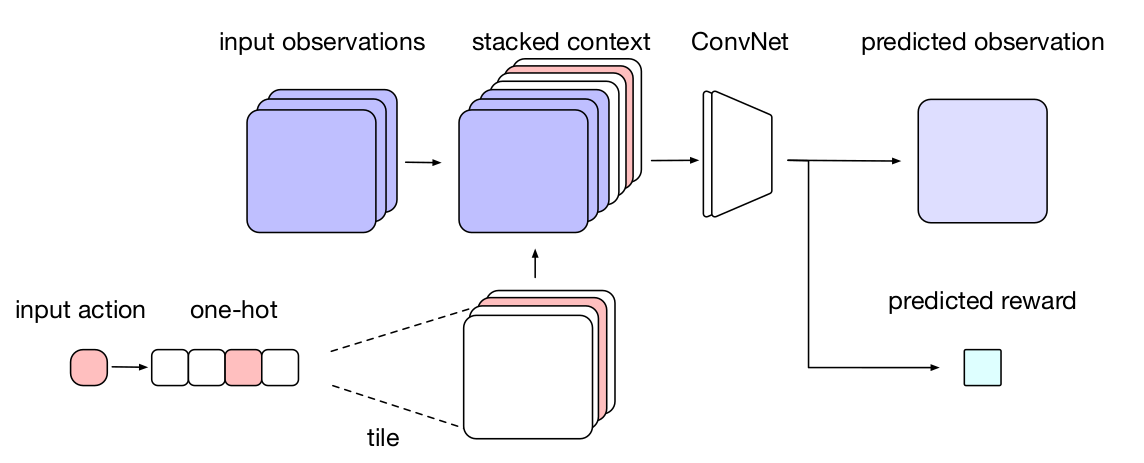
\includegraphics[width=300px]{./Images/environment_model_architecture.png}
  \caption{TODO} 
  \label{fig:environment_model_architecture} 
\end{figure} 

Figure \ref{fig:environment_model_architecture} shows the environment model architecture. It gets as input the last observation as rgb image $o_t$ and the from the rollout policy selected action $a$. The action is converted to a one hot vector and tiled to the size of the observation. The tiled action is then concatinated with the input observations. A convolutional neural network with two heads predicts then the next observation and the expected reward.\\

The neuronal network is trained with pairs of $(o_t, a_t) \rightarrow (o_{t+1}, r_{t+1})$ generated from a pretrained model-free advantage-actor-critic policy. This is nessesary because a random agent is not able to generate a representative set of states, as it sees few rewards in some of the domains.\\

 
The environment model is trained by maximize the log likelihood of the probability $p(o_t | a_{t-1}, o_{t-1})$. Where $p(o_t | a_{t-1}, o_{t-1})$ is a bernoulli distribution: 
\begin{equation} 
   p(o_t | a_{t-1}, o_{t-1}) = x^y (1-x)^{1-y} 
\end{equation} 
   
$log p(o_t | a_{t-1}, o_{t-1})$ equals to Binary Cross Entropy between the true image and the predicted imageloss 
   
\begin{equation} 
  \mathnormal{ 
  env_{loss}(x, y) = \frac{1}{N} \sum y_n log x_n + (1-y_n) log(1- x_n) 
  %env_{loss} = Binary Cross Entropy(predicted\_image, true\_images) 
  } 
  \end{equation} 
 
 
 
\subsection{Single Imagination Rollout}
 
 
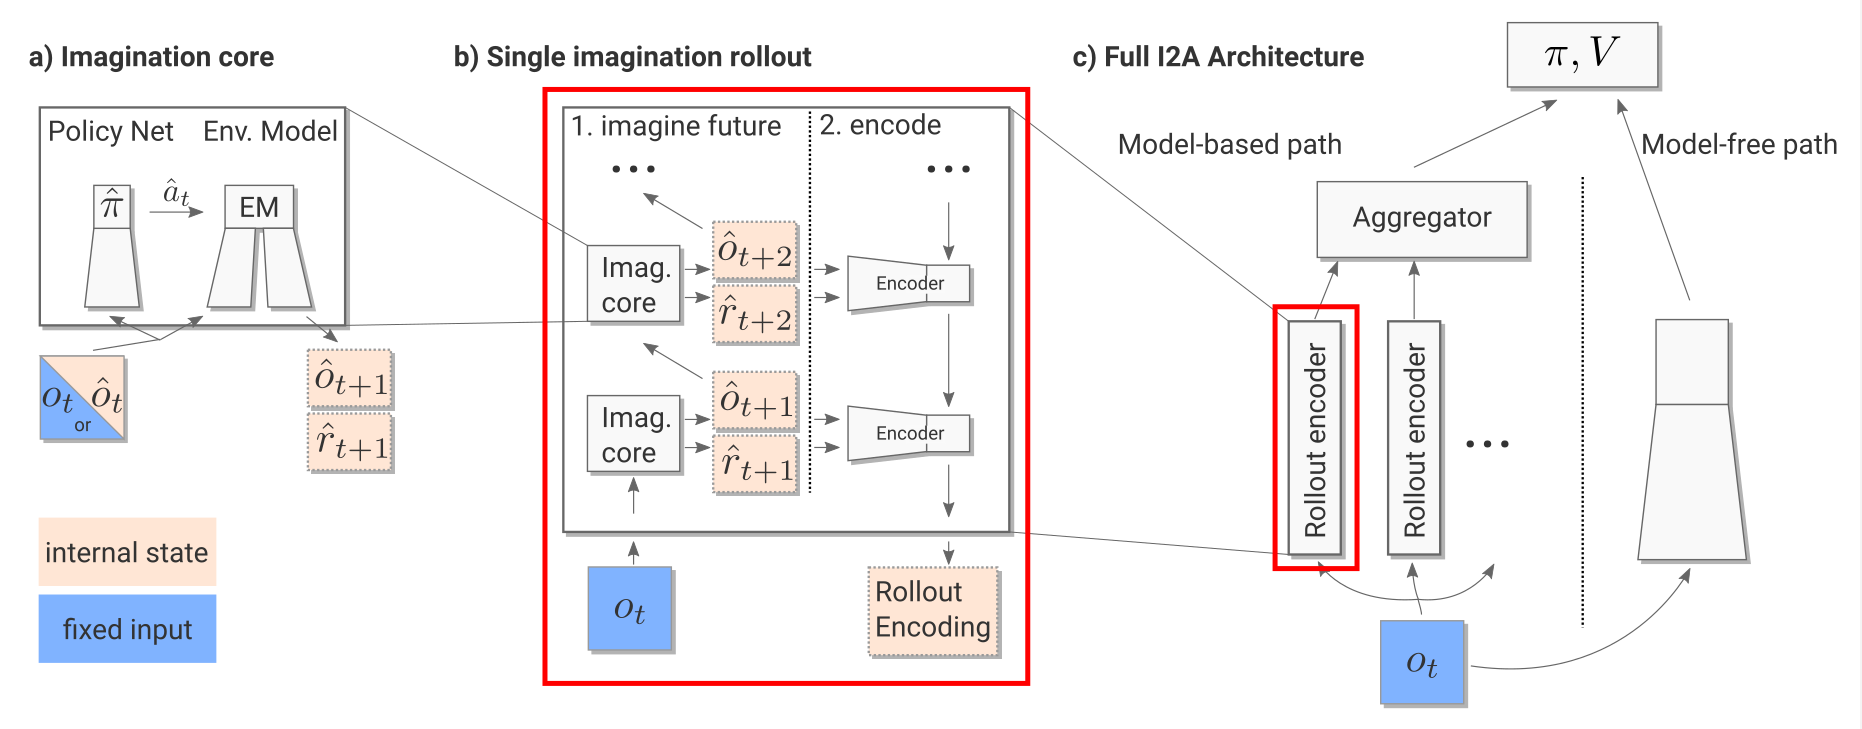
\includegraphics[width=\columnwidth]{./Images/i2a_all_imagination_rollout.png}% 
 
The imagination core imagines trajectories of features $f = (\hat{o}, \hat{r})$\\ 
The rollout encoder encode these trajectories     
 
 
 
I2A Architecture - Imagination Future 
 
Input:\\ 
    observation $o_t$ \\ 
    (1 MiniPacman frame)\\ 
    start action $a$ 
Output:\\ 
    n imagined trajectories ($\hat{o}_{t+i}, \hat{r}_{t+i}$ for $i = 0, ..., n$) 
     $\hat{} \hspace{2mm} \rightarrow$ internal state 
   
  %\begin{center} 
    %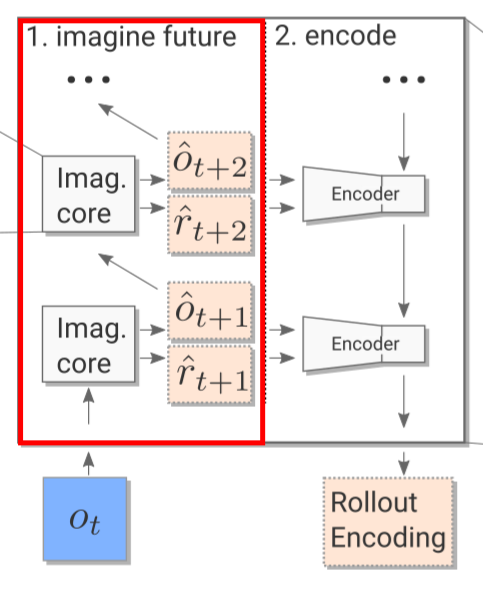
\includegraphics[height=.5\textheight]{./Images/imagine_future.png}% 
  %\end{center} 
 
I2A Architecture - Encoder 
 
     CNN Network followed by an LSTM Network 
    CNN Network:\\ 
    Encode observation and reward $\hat{o}_{t+i}, \hat{r}_{t+i}$ 
    LSTM Network:\\ 
    Learns long-term dependencies 
    %\item Learns useful information from the rollout trajectories 
   
  \begin{center} 
    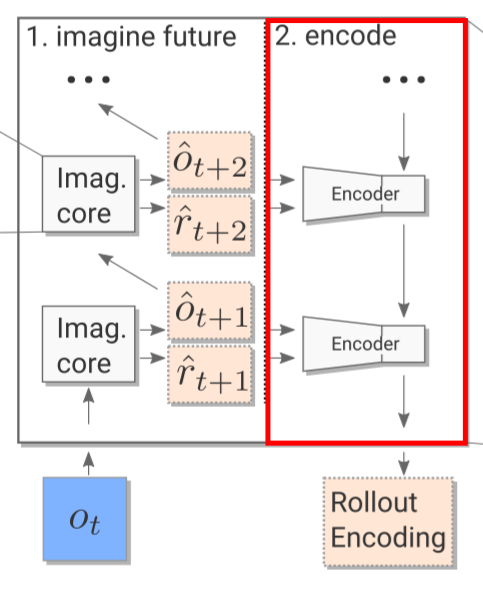
\includegraphics[height=.2\textheight]{./Images/encoder.png}% 
  \end{center} 
 
 
 
I2A Architecture - Model Based Path 
 
 
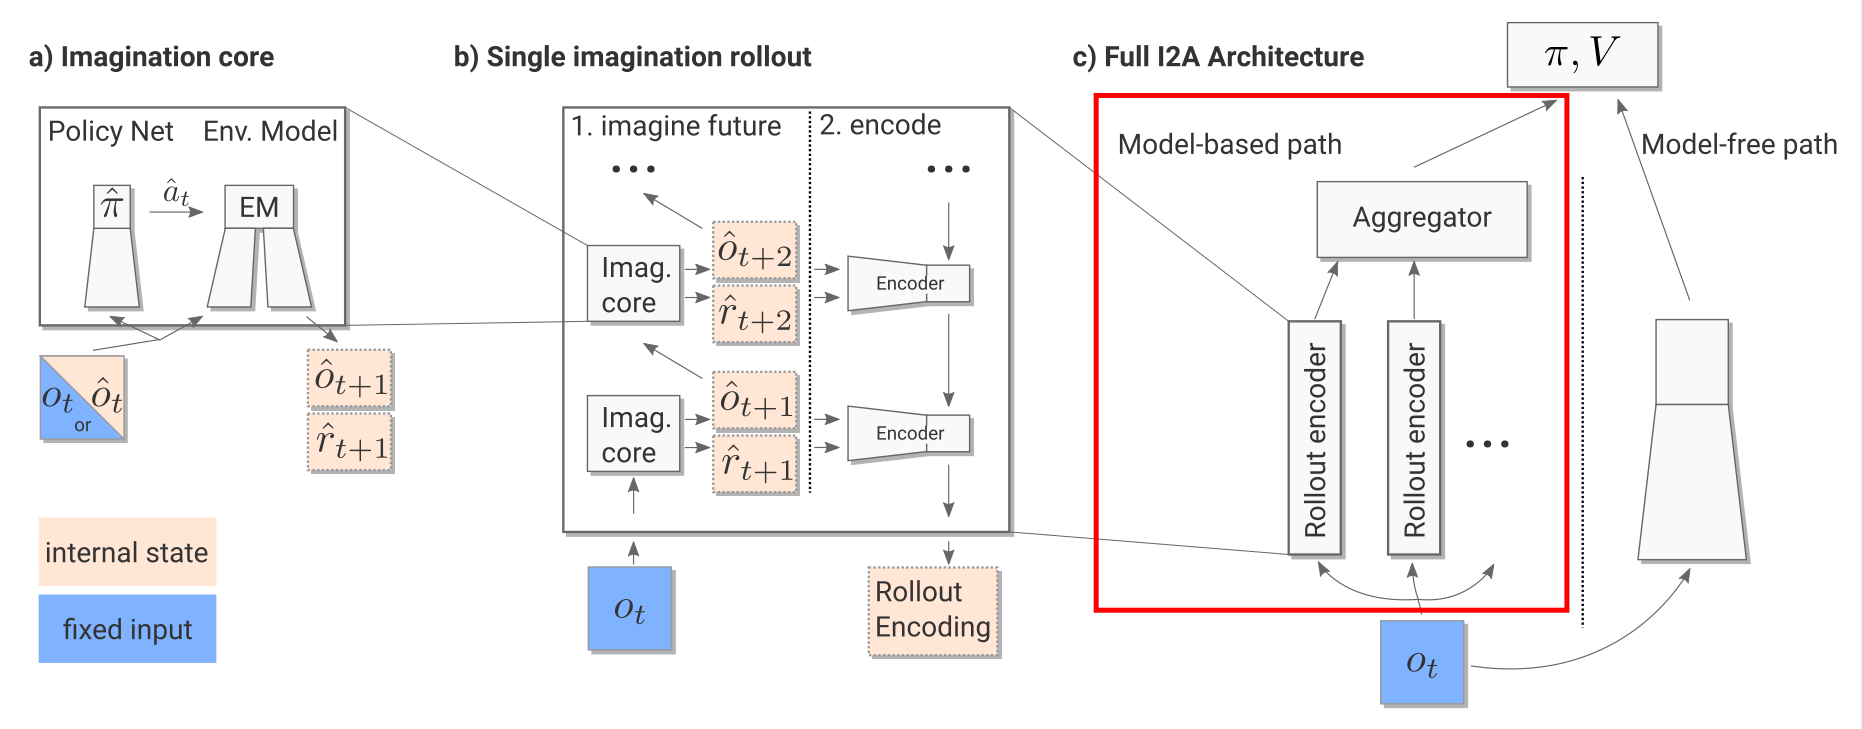
\includegraphics[width=\columnwidth]{./Images/i2a_all_model_based_path.png}% 
 
%For each action $a$ the agent can take do a imagination rollout  
% the future based on a model of the environment and use this information for decision making 
 
 
I2A Architecture - Model Based Path 
 
 
       For each action $a$ the agent can take, do a imagination rollout  
    %For each action the agent can take,  
    %imagine the future% and learn relevent information that can happen 
     Aggregator: \\ 
    Concatinate all action rollouts 
   
  %\begin{center} 
    %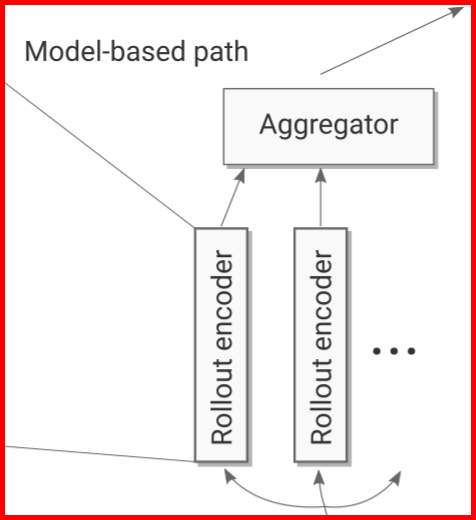
\includegraphics[height=.5\textheight]{./Images/i2a_model_based.png}% 
  %\end{center} 
 
 
 
I2A Architecture - Model Free Path 
 
 
 
CNN Layers followed by Fully Connected Layers 
 
 
 
I2A Training 
Input:\\ 
    Observation $o_t$ 
     Output:\\ 
    Policy $\pi$ and value function $V$ 
     Train with Advantage-Actor-Critic (A2C) 

